\section{Grayscale Conversion}
\label{sec:grayscale-conversion}

The Canny Edge Detection algorithm operates on grayscale images. This is because edge detection is primarily concerned with changes in intensity. Converting a color image to grayscale simplifies the computation and focuses on the luminance information, which is crucial for detecting edges.

The effect after converting a color image to grayscale is shown in \autoref{fig:color-vs-grayscale}.

\begin{figure}[ht]
    \centering
    \begin{subfigure}[b]{0.4\textwidth}
        \centering
        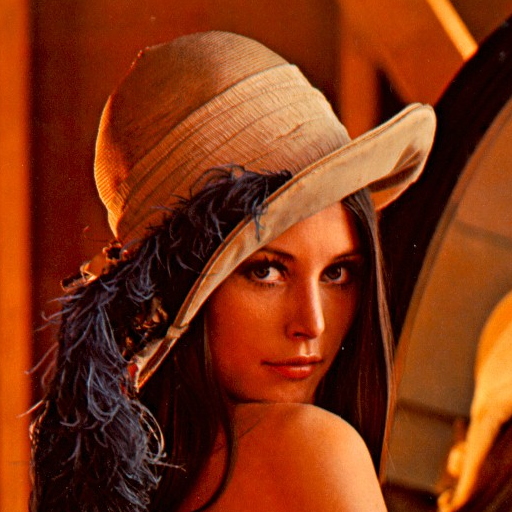
\includegraphics[width=0.9\textwidth]{lenna_1_original.png}
        \caption{Original Color Image}
        \label{fig:lena-color}
    \end{subfigure}
    \hfill
    \begin{subfigure}[b]{0.4\textwidth}
        \centering
        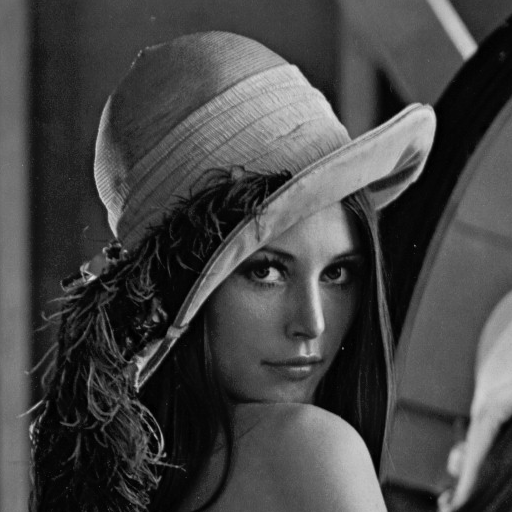
\includegraphics[width=0.9\textwidth]{lenna_2_grayscale.png}
        \caption{Grayscale Image}
        \label{fig:lena-grayscale}
    \end{subfigure}
    \caption{Output of Converting a Color Image to Grayscale}
    \label{fig:color-vs-grayscale}
\end{figure}